\documentclass[twocolumn]{article}
\usepackage{calc}
\usepackage[margin=0.5in]{geometry}
\usepackage{amsmath,amsthm,amsfonts,amssymb}
\usepackage{amsfonts}
\usepackage{color,overpic}
\usepackage{hyperref}
\usepackage{enumitem}
\usepackage{graphicx}
\usepackage{caption}
\usepackage{natbib}
\bibliographystyle{apalike}
\usepackage{framed}
\usepackage{float}

\newenvironment{Figure}
  {\par\medskip\noindent\minipage{\linewidth}}
  {\endminipage\par\medskip}
  
\numberwithin{equation}{section}


% Turn off header and footer
\pagestyle{empty}
\setlist[itemize]{leftmargin=*} % set itemise indentation to leftmargin
\setlist[enumerate]{leftmargin=*}



\title{Optimization}
\date{\vspace{-6ex}}
% -----------------------------------------------------------------------

\begin{document}
\maketitle



\section{Introduction}

	\subsection{Generality}
\begin{itemize}
	\item \textbf{Definition} flexible, transparent fiber made by  drawing\footnote{strech by forcing the material to go through a die} glass (silica) or plastic to a diameter slightly thicker than that of a human hair.
	\item \textbf{Benefit} (compare to metal wire) low loss (0.2 dB/km)\footnote{If ocean water was as clear as fiber, one could see the bottom of the Marianas Trench in the Pacific Ocean (depth of 11km)} and therefore travel longer distance, no electromagnetic inference and insolator (can be strung along with power cables), broad bandwidth
	\item Optical fibers typically include a transparent core surrounded by a transparent cladding material with a lower index of refraction. Light is kept in the core by the phenomenon of total internal reflection which causes the fiber to act as a waveguide. (see below for more explanation)
	\item Fibers that support many propagation paths or transverse modes are called multi-mode fibers (MMF).
	\item Joining two optical fiber involves cleaving of the fibers, perfect alignment of the fiber cores, and the splicing of these aligned fiber cores.
\end{itemize}

	\subsection{History and Development}
\begin{itemize}
	\item Guiding of light by refraction, the principle that makes fiber optics possible, was first demonstrated by Daniel Colladon and Jacques Babinet in Paris in the early 1840s. John Tyndall included a demonstration of it in his public lectures in London, 12 years later.
	\item Image transmission through tubes was demonstrated independently by the radio experimenter Clarence Hansell and the television pioneer John Logie Baird in the 1920s.
	\item The first working fiber-optical data transmission system was demonstrated by German physicist Manfred Börner at Telefunken Research Labs in Ulm in 1965, which was followed by the first patent application for this technology in 1966.
	\item NASA used fiber optics in the television cameras that were sent to the moon.
	\item The 2009 Nobel Prize in Physics was awarded to Charles K. Kao for his theoretical work on the single-mode optical fiber
\end{itemize}

	\subsection{Uses}
\begin{itemize}
	\item \textbf{Communication.} The typical per-channel light signals propagating rate is between 10 40 Gbit/s in deployed systems but in 2013, researchers have reach 400 Gbit/s.
	\item \textbf{Sensing.} measure strain, temperature, pressure and other quantities by modifying a fiber so that the property to measure modulates the intensity, phase, polarization, wavelength, or transit time of light in the fiber.
	\item \textbf{Power transmission.} Optical fiber can be used to transmit power using a photovoltaic cell to convert the light into electricity
	\item light guiding, Optical fiber lamp, fiberscope, shotguns use pieces of optical fiber to improve visibility of markings on the sight.
\end{itemize}


	\subsection{Manufacturing}
Glass optical fibers are almost always made from silica ($n=1.5$). Typically the index difference between core and cladding is less than one percent.

Plastic optical fibers (POF) are commonly step-index multi-mode fibers with a core diameter of 0.5 millimeters or larger and have higher attenuation coefficients than glass fibers (1 dB/m).

Fusion splicing and cleaving of silica fibers is relatively effective.
 
 Silica fiber also has high mechanical strength against both pulling and even bending, provided that the fiber is not too thick and that the surfaces have been well prepared during processing.

Optical fibres are made from doped quartz glass. Quartz glass is a form of silicon dioxide (SiO2) with amorphous solid structure.


\section{Physic}
	\subsection{Optical law behind}
The \textbf{refractive index} is a dimensionless number that describes how light propagates through that medium: $n=\frac{\mathrm{c}}{v}$
where c is the speed of light in vacuum ($~3\times 10^8 [m/s]$) and v is the phase velocity of light in the medium. Typical value: 1 (air), 1.33 (water), 1.5-1.6 (glass), 2.42 (Diamond) 


\textbf{Snell's law} describe the relationship between the angles of incidence and refraction of a waves passing through a boundary between two different isotropic media. The law follows from Fermat's principle\footnote{The path taken between two points by a ray of light is the path that can be traversed in the least time.} of least time.
$$\frac{\sin\theta_1}{\sin\theta_2} = \frac{v_1}{v_2} = \frac{\lambda_1}{\lambda_2} = \frac{n_2}{n_1}$$
with each $\theta$ as the angle measured from the normal of the boundary and $\lambda$ as the wavelength of light in the medium. 
\begin{figure}[H]
	\centering
	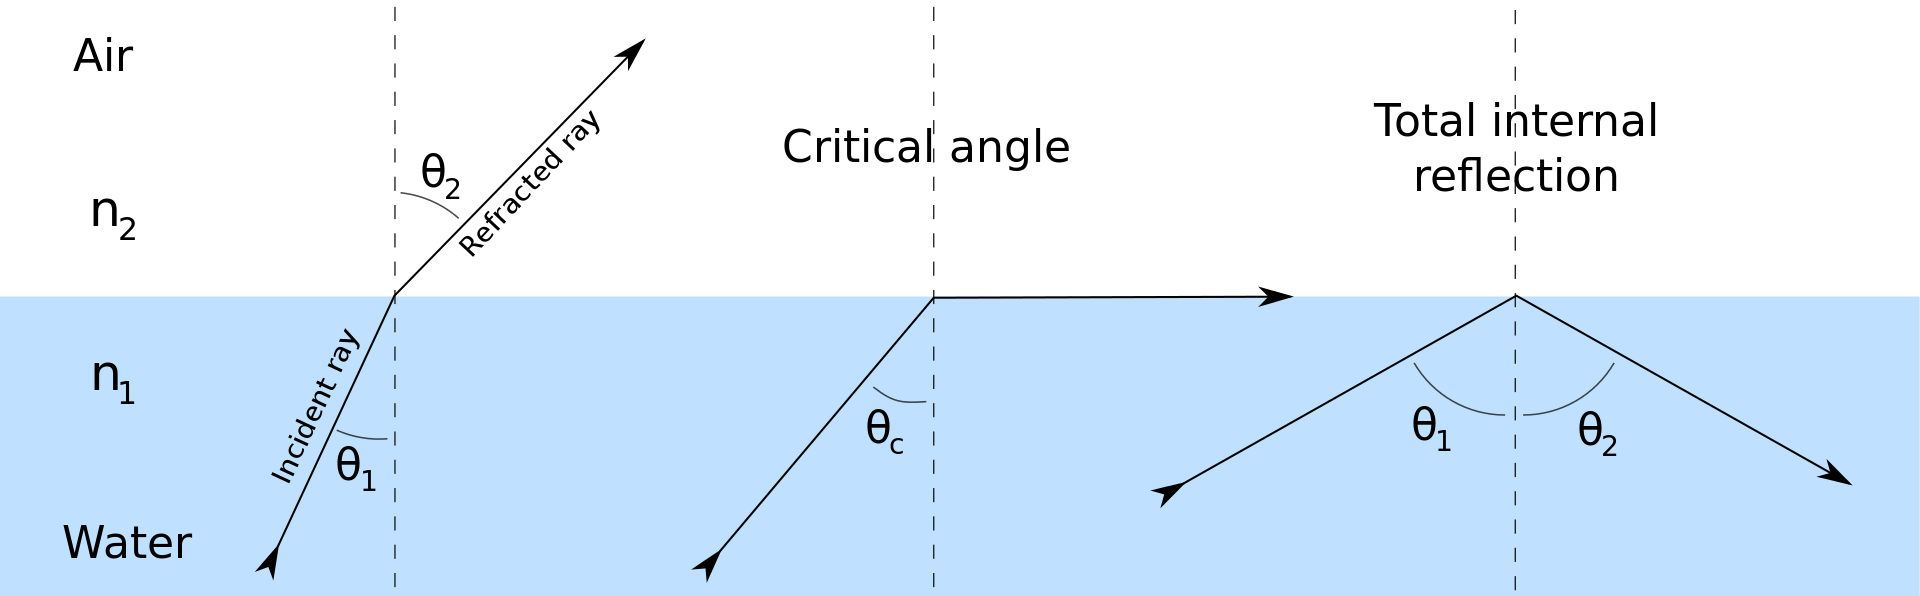
\includegraphics[width=.5\textwidth]{1920px-RefractionReflextion.png}
\end{figure}

The \textbf{critical angle} of incidence $\theta_\text{crit}$ is encounter when the refracted angle $\theta_2=\pi/2$ ($\sin\theta_2=1$).
$$\theta_1 = \theta_\text{crit} \text{ if } \theta_2=\pi/2 \Rightarrow \theta_\text{crit}=\arcsin\left(\frac{n_2}{n_1}\right)$$

\textbf{Total internal reflection} occurs when the incidental angle is larger than the critical angle. In this situation, the wave cannot pass through and is entirely reflected. This can only occur for $n_1>n_2$

	\subsection{Principle of operation}
The optic fiber uses the total internal reflection phenomenon to confine the light in the fiber. The fiber is a cylindrical dielectric waveguide that consist of a cladding is a layer of lower refractive index than a core material. 

The Sin of the maximal acceptance angle is called the \textbf{Numerical Aperture (NA)}. Fiber with a large NA requires less precision to splice. However, a large acceptance cone increases the amount of dispersion as rays at different angles take different times to traverse the fiber.
$$\mathrm{NA}=\sqrt{n_\mathrm{core}^2-n_\mathrm{clad}^2}$$

\begin{figure}[H]
	\centering
	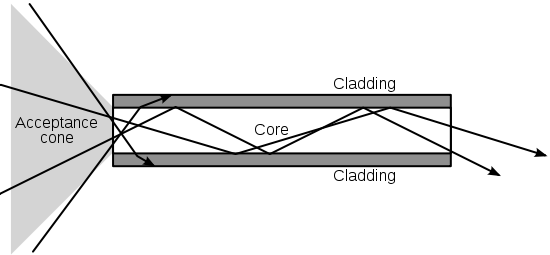
\includegraphics[width=.5\textwidth]{550px-Optical-fibre.png}
\end{figure}


	\subsection{Attenuation}
\begin{itemize}
	\item \textbf{Diffuse reflection} (or scattering) is cause by  molecular level irregularities making light rays to be reflected in random directions. Light scattering depends on the wavelength of the light being scattered.
	\item signal loss can also occur due to selective absorption of specific wavelengths.
\end{itemize}
\begin{figure}[H]
	\centering
	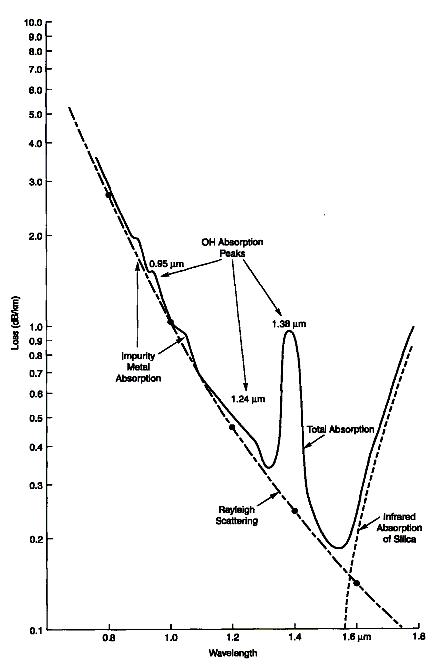
\includegraphics[width=.25\textwidth]{Fibre-Optic-Spectral-Attenuation-Graph.png}
\end{figure}
More definiton for modeling attenuation:
\begin{itemize}
	\item \textbf{radiant energy}, the energy of an electromagnetic radation ($Q_e$ [J]=[kg m\textsuperscript{2}/s\textsuperscript{2}]) 
	\item \textbf{radian flux} is the flux of this energy and therefore the power ($\Phi_\mathrm{e} = \frac{\partial Q_\mathrm{e}}{\partial t}$ in [W] or [J/s]). 
	\item The \textbf{transmittance} $T$ of material sample relate the incident ($^i$) and transmitted ($^t$) radiant flux : $T = {\Phi_\mathrm{e}^\mathrm{t}}/{\Phi_\mathrm{e}^\mathrm{i}}$
	\item \textbf{optical depth} $\tau$ ([-]) or \textbf{absorbance} $A$ ([-])are related to transmittance with : $T = e^{-\tau} = 10^{-A}$
where  is the by that material sample and $\Phi_\mathrm{e}^\mathrm{i}$ is the radiant flux  by that material sample.
	\item The \textbf{molar attenuation coefficient} ($\epsilon$ [m\textsuperscript{2}/mol]) is a measurement of how strongly a chemical species attenuates light at a given wavelength
	\item \textbf{The Beer-Lambert} law relates the attenuation of light to the properties of the material:
	$$A = \sum_{i = 1}^N A_i = \sum_{i = 1}^N \varepsilon_i \int_0^\ell c_i(z)\,\mathrm{d}x$$
	with, material of length $l$ is compose of $i$ species of molar concentration $c_i$.
\end{itemize}



	\subsection{Index Fiber}
\begin{itemize}
	\item Step-index fiber have abrupt boundary between the core and cladding. 
	\item In graded-index fiber uses a continuous decreasing index of refraction between core and cladding. The light ray bound smoothly and reduce the dispersion because high angle rays pass more through the lower-index periphery of the core, rather than the high-index center.
\end{itemize}


	\subsection{Mode}
In such case, traditional geometric optics don't apply and solving Helmholtz equation ($\nabla^2 A + k^2 A = 0$,  $k$ is the wavenumber, and $A$ is the amplitude. Maxwell's equation combined with the boundary condition) gives the modes (how the wave is distributed in space).
Mode is a particular ray light travelling at a particular angle.
$$v=\frac{2\pi}{\lambda_0}d_c\sqrt{n_1^2-n_2^2}$$
\begin{figure}[H]
	\centering
	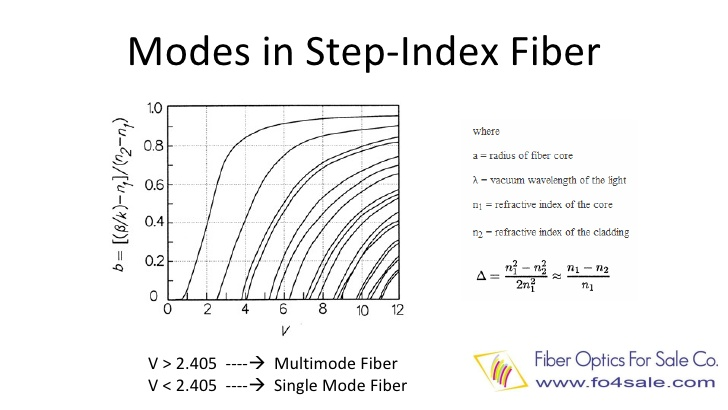
\includegraphics[width=.5\textwidth]{what-is-single-mode-and-multimode-fiber-4-728.jpg}
	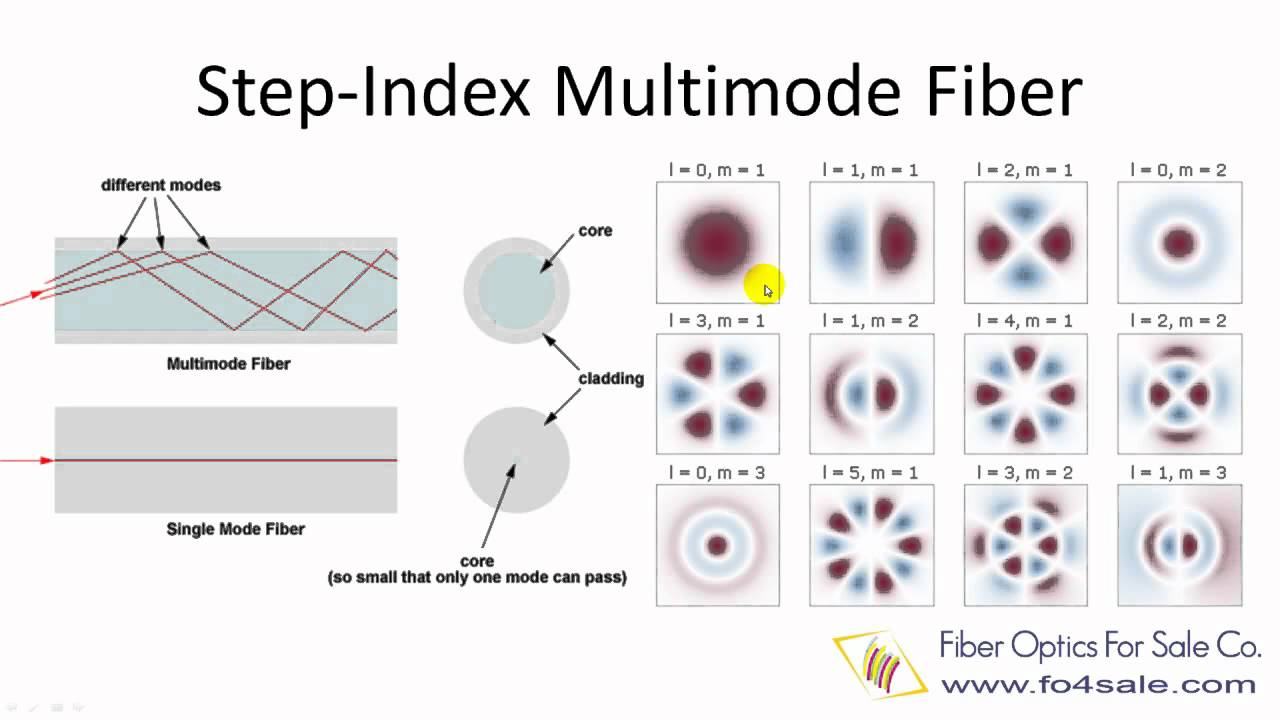
\includegraphics[width=.5\textwidth]{maxresdefault.jpg}
\end{figure}

\begin{itemize}
	\item \textbf{Multi-mode fiber} are fiber with large core diameter which are analysed by geometrical optics (as explain before). 
	\item \textbf{Single-mode} have a core diameter less than ten times the wavelength of the propagating light.  Single-mode optical fibers have only one solution and therefore a single ray which make extremely low loss.
	\item Special-purpose fiber
\end{itemize}

\begin{figure}[H]
	\centering
	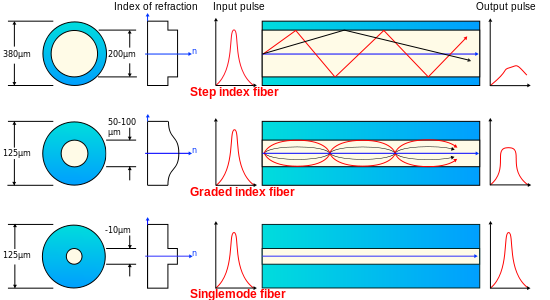
\includegraphics[width=.5\textwidth]{550px-Optical_fiber_types.png}
\end{figure}


	\subsection{Fermi-Dirac and Bose-Einstein statistics, Maxwell Boltzmann statistics}

Gibbs paradox :...

Quantum particles are either bosons (following instead Bose–Einstein statistics) or fermions (subject to the Pauli exclusion principle, following instead Fermi–Dirac statistics). 

		\subsubsection{Maxwell-Boltzmann statistics}
The expected number of particles with energy $\varepsilon_i$ for Maxwell–Boltzmann statistics is $\langle N_i \rangle$ where:
$$\langle N_i \rangle = \frac {1} {e^{(\varepsilon_i-\mu)/kT}} = \frac{N}{Z} e^{-\varepsilon_i/kT}$$
where $N$ is the total number of particles $N=\sum_i N_i$ and $Z$ is the partition function $Z=\sum_i e^{-\varepsilon_i/kT}$. 
Boltzmann constant is a physical constant relating energy at the individual particle level $E$ with temperature $T$. It is also equal to the gas constant $R$ divided by the Avogadro constant $N_A$:
$$k = \frac{E}{T} = \frac{R}{N_\text{A}} = 1.38\times 10^{−23} [J/K]$$
Maxwell-Boltzmann statistics is only valid when $e^{(\varepsilon_{\rm min}-\mu)/kT} \gg 1$


		\subsubsection{Fermi–Dirac statistics}
		
$$\langle N_i \rangle = \frac{1}{e^{(\varepsilon_i-\mu)/kT}+ 1}$$


		\subsubsection{Bose-Einstein statistics}

$$\langle N_i \rangle = \frac{1}{e^{(\varepsilon_i-\mu)/kT}-1}$$




\newpage
\section{Scattering}
	\subsection{Introduction}
		\subsubsection{Light}
\begin{itemize}
	\item Visible light is an electromagnetic radiation which have a wavelength comprise between 400nm (violet) and 700nm (red).
	\item Its properties include: intensity, propagation direction, frequency (or wavelength), and polarisation.
	\item It has the fastest speed possible : $3\times 10^8 [m/s]$ and it always travel at this speed (idpdt of medium).
	\item Usual wave needs a medium to travel (sound is a compression of air particle) but light don't need one.
\end{itemize}
	
		\subsubsection{Quantum theory}
In 1900 Max Planck, attempting to explain black body radiation suggested that light could gain or lose energy by finite amounts (called quanta) related to their frequency:
$$ E = h \nu$$
In 1905, Albert Einstein used the idea of light quanta to explain the photoelectric effect. In 1926 Gilbert N. Lewis named these light quanta particles photons.
 
The modern theory of quantum mechanics sees light as something that can be described sometimes with wave theory and sometimes with particle, but is actually something that cannot be fully imagined. (see particle-wave duality)

	\subsection{Generality}
\begin{itemize}
	\item Scattering is the process where a radiation are forced to deviate due to non-uniformities in the medium through which they pass.
	\item Elastic scattering implies that the internal states (energy, wavelength) of the scattering particles do not change while in inelastic scattering the particles' internal state is changed
	\item Scattering can be divided into three domains based on the circumference of a particle ($\pi D_\text{p}$) and the wavelength ($\lambda$) of incident radiation:
	\begin{itemize}
		\item $\alpha \ll 1$: Rayleigh scattering
		\item $\alpha \approx 1$: Mie scattering
		\item $\alpha \gg 1$: geometric scattering
	\end{itemize}
	\begin{figure}[H]
	\centering
	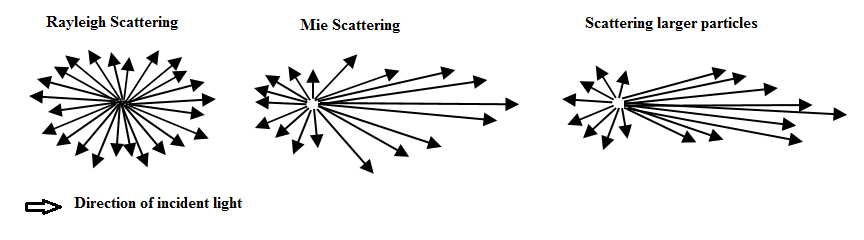
\includegraphics[width=.5\textwidth]{image11.png}
\end{figure}	
	\item In fiber optic the three major scattering are: Rayleigh, Brillioun, and Raman scattering which will be explain in more detail below
\end{itemize}


	\subsection{Rayleigh}
Rayleigh scattering (elastic scattering) occur when particles are much smaller than the wavelength of the radiation $(d < 1 /10 \lambda$). In optic fiber, the energy losses coefficient ($I/I_0$) is 
$$\alpha_\text{scat} = \frac{8 \pi^3}{3 \lambda^4} n^8 p^2 k T_\text{f} \beta$$
where $n$ is the refraction index, $p$ is the photoelastic coefficient of the glass, $k$ is the Boltzmann constant, and $\beta$ is the isothermal compressibility. $T_f$ is a fictive temperature, representing the temperature at which the density fluctuations are ``frozen'' in the material. The strong wavelength dependence ($~\lambda^{−4}$) means that shorter (blue) wavelengths are strongly scattered (explaining the blue sky).


	\subsection{Raman scattering}
Raman scattering is an inelastic scattering meaning that scattered photon have lower frequency than the incidental one. This only concerne a very small fraction of the scattered photons (approximately 1 in 10 million). The difference in energy (related to the frequency shift) between the excitation and scattered photons corresponds to the energy required to excite a molecule to a higher  or lower vibrational mode:
\begin{itemize}
	\item Stokes (red-shifted): lower energy than the absorbed photon.
	\item anti-Stokes (blue-shifted): higher energy than the absorbed photon.
\end{itemize}
The relative amplitude of the two signals (Stokes and anti-Stokes) varies with temperature, while their wavelength is independent of temperature.
\begin{figure}[H]
	\centering
	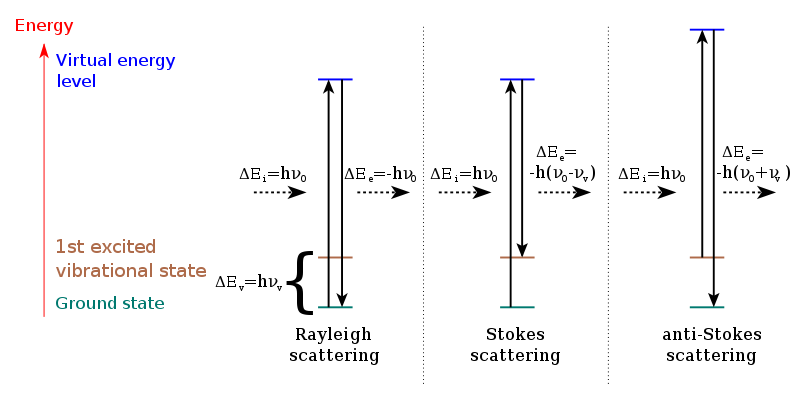
\includegraphics[width=.5\textwidth]{800px-Ramanscattering.png}
\end{figure}
The Raman Stokes signal is generated when a photon excites a vibrating molecule at a base excitation state and the molecule returns to a slightly higher vibrational state.	The anti-Stoke is created when the molecule excitation state is higher than the incoming photon. The warmer the medium is, the more frequently these previously-excited molecules will be encountered and the ratio Stoke-anti-Stoke is low.

\begin{enumerate}

\item According to Beer's law, the power of a signal  decrease exponentially with distance:
$$P(z) = P_0 \exp (-\tau) = P_0 \exp (-\int_0^z \alpha(z') dz')$$
Which for uniform attenuation is simplify to
$$P(z) = P_0 \exp (-\alpha z)$$


\item The power of the back-scattering of Stokes and anti-Stokes signals ($P_{AS}$ and $P_S$, respectively) from a short section $\Delta z$ of fiber is given by:
 $$\Delta P_{AS}(z) = \text{Pr}_{AS} \Gamma_{AS} P(z) \Delta z \quad \text{and} \quad \Delta P_{S}(z) = \text{Pr}_{S} \Gamma_{S} P(z) \Delta z $$	
where $\Gamma$ is the fraction of the scattered light that is directed back into the fiber towards the initial light source (capture coefficients, vary with medium) and $P(z)$ is the incident laser pulse power. 

We can then integrate the previous equation:
$$ \int \frac{\Delta P_{AS}}{\Delta z} d z= \int \text{Pr}_{AS} \Gamma_{AS} P_0 \exp (-\alpha z)dz $$
$$ P_{AS}(z)= \text{Pr}_{AS} \Gamma_{AS} P_0 \frac{1}{\alpha}\exp (-\alpha z)$$

But we are measuring the back-scatter once they are back to the instrument, thus the signal is again attenuated :

$$ P_{AS}^{meas}(z)= P_{AS}(z) \exp (-\alpha_{AS} z)= \text{Pr}_{AS} \Gamma_{AS} P_0 \frac{1}{\alpha}\exp (-\alpha z)\exp (-\alpha_{AS} z)$$
where $\alpha_{AS}$ is the attenuation coefficient for the anti-Stokes as opposed to $\alpha$ which the the attenuation for the pure signal.

We can do the same for the stokes and take the ratio of both:

\item In the anti-Stokes process, the scattering annihilates a phonon and is proportional to the average phonon number given by Bose-Einstein statistics are:
$$ \text{Pr}_{S} = \langle N_i \rangle=  \frac{1}{1-\exp\left(\frac{-\Delta E}{kT}\right)}$$ 
For the Stokes  process, the scatering creates a phonon and the commutation rule of the quantum annihilation-creation operators makes the cross-section proportional to 

$$ \text{Pr}_{AS} = 1 +\langle N_i \rangle=\frac{\exp\left(\frac{-\Delta E}{kT}\right)}{1-\exp\left(\frac{-\Delta E}{kT}\right)}$$  
 where $T$ is the temperature of the fiber at the point of scattering, $\Delta E$ is the frequency shift between the incident light and the scattered Raman signals, and $k$ is the Boltzmann constant. 

\item The ratio $\frac{\Gamma_{AS}}{\Gamma_{S}}$ can be approximated by the wavelenghts to the power 4. I don't know why...
\item The DTS instrument receptor has a relative efficiencies to detect Stokes and anti-Stokes. In order to take that for account we need to add a $R$ term
\item Bringing all that together
$$\frac{P_{AS}^{meas}}{P_{S}^{meas}}(z)=\frac{R_{AS}}{R_S}\exp\left(\frac{-\Delta E}{kT}\right) \left( \frac{\lambda_{AS}}{\lambda_{S}}  \right)^4 \exp (-\Delta  \alpha z)$$
\item Solving for $T$
$$T = \frac{\Delta E/k}{\ln\frac{P_S}{P_{AS}} + \ln\frac{R_{AS}}{R_{S}} + \ln\left[\left(\frac{\lambda_S}{\lambda_{AS}}\right)^4\right] - \Delta\alpha z}$$

\item Which is simplify with empirical/calibrated parameter:
$$ T(z) = \frac{\gamma}{\ln\frac{P_S(z)}{P_{AS}(z)} + C - \Delta\alpha z}$$


Or, the assumption of constant attenuation and time independence can be removed :

$$ T(z,t) = \frac{\gamma}{\ln\frac{P_S(z,t)}{P_{AS}(z,t)} + C(t) - \int_0^z \alpha(z') dz'}$$

where:
\begin{itemize}
 \item $T(z,t)$ is the temperature (K) 
 \item $z$ is the distance along the cable with $z$ = 0 at the DTS instrument  
 \item $P_{S}(z,t)/P_{aS}(z,t)$ is the measured ratio between the power of the  Stokes (S) and anti-Stokes (aS) backscatter reaching the instrument.
 \item $\gamma = \DeltaE/ k = h \Omega / k$, where $h$ is the Planck’s constant, $\Omega$  is the difference in frequency between the backscattered Stokes radiation and the incoming laser pulse and $k$ is Boltzmann’s constant. Often  treated as a constant $\gamma$ can show changes as a function of the instrument temperature and power supply. 
 \item $C(t)=\ln\frac{R_{AS}}{R_{S}} + \ln\left[\left(\frac{\lambda_S}{\lambda_{AS}}\right)^4\right]$ accounts for the differences in effective detector sensitivities with respect to Stokes and anti-Stokes photons, which may  vary in time ( caused by thermal sensitivity of the detectors, as well as thermal variation in the alignment of the optical system.)
  \item $\int_0^z \Delta \alpha(z') dz'$ represents the differential attenuation of the Stokes and anti-Stokes radiation caused by the differences in the absorption coefficients for both  frequencies. When the differential attenuation is uniform along a cable,  the value of $\Delta \alpha(z)$ in the denominator is constant and the  integral in the denominator simplifies to $\Delta \alpha \times z$. Note  that attenuation can be a function of temperature but in general, one  does not expect $\Delta \alpha$ to change rapidly in time if the cable’s  position and environment does not change rapidly. It can also be affected by the selection and the physical condition of the optical fiber itself. 
\end{itemize}
\end{enumerate}




	\subsection{Brillouin Scattering}
The result of the interaction between the light-wave and the carrier-deformation-wave is that a fraction from the passing-through light-wave changes its momentum (thus its frequency and energy) along preferential angles, as if by being diffracted by an oscillating 3-D grating.
In Brillioun scattering, the amplitudes of the Stokes and anti-Stokes signals are predictable given the amplitude of the incident light, but the wavelengths of the resulting signals are variable 





	\subsection{Fiber Bragg grating (FBG)}
It is a type of distributed Bragg reflector constructed in a short segment of optical fiber that reflects particular wavelengths of light and transmits all others. This is achieved by creating a periodic variation in the refractive index of the fiber core, which generates a wavelength-specific dielectric mirror. A fiber Bragg grating can therefore be used as an inline optical filter to block certain wavelengths, or as a wavelength-specific reflector.
\begin{figure}[H]
	\centering
	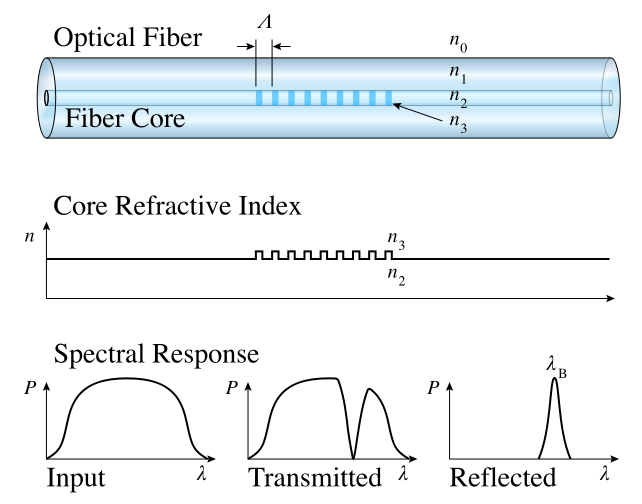
\includegraphics[width=.5\textwidth]{642px-Fiber_Bragg_Grating-en.png}
	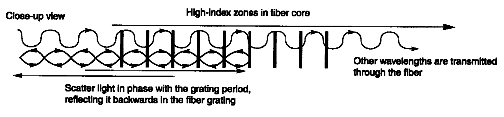
\includegraphics[width=.5\textwidth]{1bf87a87405.png}
\end{figure}

The fundamental principle behind the operation of an FBG is Fresnel reflection,where light traveling between media of different refractive indices may both reflect and refract at the interface.

The refractive index will typically alternate over a defined length. The reflected wavelength ($\scriptstyle \lambda_B$), called the Bragg wavelength, is defined by the relationship,

$$\lambda_B = 2 n_e \Lambda$$
where $\scriptstyle n_e$ is the effective refractive index of the grating in the fiber core and $\scriptstyle \Lambda$ is the grating period. The effective refractive index quantifies the velocity of propagating light as compared to its velocity in vacuum. $\scriptstyle n_e$ depends not only on the wavelength but also (for multimode waveguides) on the mode in which the light propagates










\newpage
\section{Distributed Temperature Sensing (DTS)}
Distributed temperature sensing systems (DTS) are optoelectronic devices which measure temperatures by means of optical fibres functioning as linear sensors.
Typically the DTS systems can locate the temperature to a spatial resolution of 1 m with accuracy to within ±1°C at a resolution of 0.01°C for distences greater than 30km.


While Brillioun-based DT instruments are commercially available [1], the Raman-based systems are more commonly used in hydrology because of the greater temperature accuracies that can be attained.


\subsection{Optical Time vs Frequency Domain Reflectometry}
There are two basic principles of measurement for distributed sensing technology, OTDR (Optical Time Domain Reflectometry) and OFDR (Optical Frequency Domain Reflectometry).

OTDR was developed more than 20 years ago and has become the industry standard for telecom loss measurements which detects the—compared to Raman signal very dominant—Rayleigh backscattering signals. The principle for OTDR is quite simple and is very similar to the time of flight measurement used for radar. Essentially a narrow laser pulse generated either by semiconductor or solid state lasers is sent into the fibre and the backscattered light is analysed. From the time it takes the backscattered light to return to the detection unit it is possible to locate the location of the temperature event.

Alternative DTS evaluation units deploy the method of Optical Frequency Domain Reflectometry (OFDR). The OFDR system provides information on the local characteristic only when the backscatter signal detected during the entire measurement time is measured as a function of frequency in a complex fashion, and then subjected to Fourier transformation. The essential principles of OFDR technology are the quasi continuous wave mode employed by the laser and the narrow-band detection of the optical back scatter signal. This is offset by the technically difficult measurement of the Raman scatter light and rather complex signal processing, due to the FFT calculation with higher linearity requirements for the electronic components.



\newpage
\section{Calibration}
Reason for inaccuracy: (1) instrument’s operating temperature, (2) quality and consistency of the power supply, (3) the cleanliness and physical condition of any optical connections, and (4) localized strains or bends in the fiber. Recall equation :
$$ T(z) = \frac{\gamma}{\ln\frac{P_S(z)}{P_{AS}(z)} + C - \Delta\alpha z}$$
see ... for desicussion.

\begin{figure}[H]
	\centering
	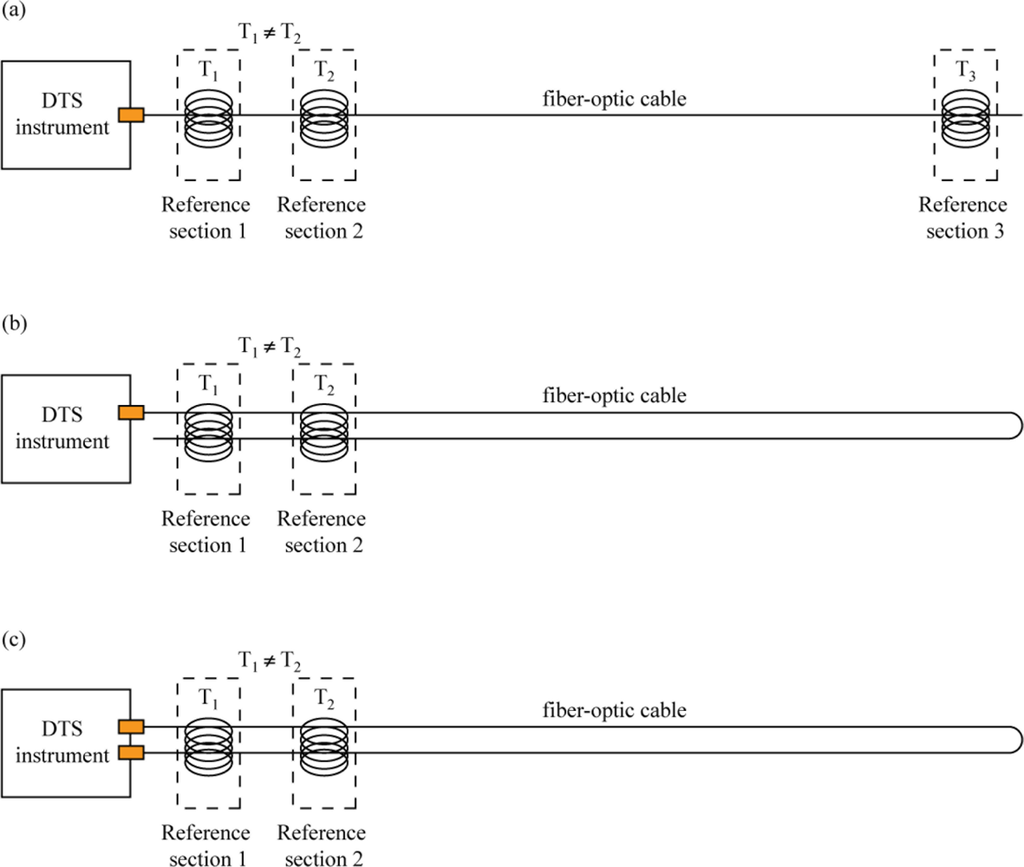
\includegraphics[width=.5\textwidth]{sensors-11-10859f1-1024.png}
\end{figure}

\section{Reference Points vs Reference Section}
It is common practice to use reference section, an average of the properties over a certain lenght (suggested by Tyler et al, to be at least 10 times the sampling inverval)
$$z^*=\frac{1}{n} \sum_{i=1}^n z_i \text{ and } {\ln\frac{P_S}{P_{AS}}}^*=\frac{1}{n} \sum_{i=1}^n \ln\frac{P_S(z_i)}{P_{AS(z_i)}}$$

\subsection{Single-ended DTS}
Single-ended calibration algorithms assume that the calibration parameters remain uniform over the entire length of the fiber.
	\subsubsection{Direct Method: 3 Temp.}
We can rearrange the equation in a linear system with the 3 parameters as unknown and use 3 differents known temperature location to solve it:
$$
\begin{bmatrix}
 1 & -T_1 & T_1z_1\\ 
 1 & -T_2 & T_2z_2\\
 1 & -T_3 & T_3z_3
 \end{bmatrix}
 \begin{bmatrix}
 \gamma\\ 
 C\\
 \Delta \alpha
 \end{bmatrix}
 =
 \begin{bmatrix}
 T_1 - \ln \frac{P_S(z_1)}{P_{AS}(z_1)}\\ 
 T_2 - \ln \frac{P_S(z_2)}{P_{AS}(z_2)}\\
 T_3 - \ln \frac{P_S(z_3)}{P_{AS}(z_3)}
 \end{bmatrix}
$$


	\subsubsection{Direct Method: 2 Temp.}
If $T$ is constent between $z$ and $z+\Delta z$, we can rearrange the equation :
$$ \ln\frac{P_S(z)}{P_{AS}(z)}  = \frac{\gamma}{T} - C + \Delta\alpha z$$
And taking the ratio at two different location result in
$$ \ln\frac{P_S(z+\Delta z)}{P_{AS}(z+\Delta z)} -\ln\frac{P_S(z)}{P_{AS}(z)} = \Delta\alpha (z+\Delta z) - \Delta\alpha z = \Delta\alpha \Delta z$$
 Solving for $\Delta \alpha$:
$$\Delta \alpha=\frac{ \ln\frac{P_S(z+\Delta z)}{P_{AS}(z+\Delta z)} -\ln\frac{P_S(z)}{P_{AS}(z)}}{\Delta z}$$

Then, the solution of the direct method can be employ to solve $\gamma$ and $C$.




\subsection{Double-ended DTS}

\subsection{Step loss}
Step losses (damage to the fibers, fusin splices...) can be handled in simple single-ended deployments by calibrating the sections of fiber on either side of the loss separately, but duplexed single-ended and double-ended methodologies both offer the potential to correct for non-uniform attenuation along the cable and are preferred whenever feasible for this reason.







\newpage
\nocite{*}
\bibliography{Fiber_Optic}	
	

\end{document}
